\documentclass{article}
\usepackage{amsmath}
\usepackage{amssymb}
\usepackage{esvect}
\usepackage[usenames, dvipsnames]{color}
\usepackage{fancyhdr}
\usepackage{hyperref}
\usepackage{pgfplots}
\usepackage{tikz}
\usepackage{geometry}
\usepackage[normalem]{ulem}

\geometry{letterpaper, portrait, margin=0.5in}
\pagestyle{fancy}

\fancyhf{} % clear all header fields
\renewcommand{\headrulewidth}{0pt}
\fancyfoot[LE,RO]{\thepage}           % page number in "outer" position of footer line
\fancyfoot[RE,LO]{\copyright\;aquarc 2025. \href{https://aquarc.org}{\underline{aquarc.org}}} % other info in "inner" position of footer line

\definecolor{myred1}{RGB}{255, 0, 0}
\definecolor{myyellow1}{RGB}{255, 255, 219}
\definecolor{mygreen1}{RGB}{0, 255, 0}
\definecolor{mygreen2}{RGB}{0, 126, 0}
\definecolor{myblue1}{RGB}{0, 0, 255}

\begin{document}

\fontsize{14}{16}\selectfont

% center the title
\begin{center}
    \textbf{\underline{Theorems Cheatsheet}}
\end{center}

\section{Fundamental Theorem of Calculus}

Part 1:

\begin{align*}
    F(x)=\int_a^x{f(t)dt} \\
    F'(x)=f(x)
\end{align*}

Part 2:

\begin{align*}
    \int_a^b f'(x)dx = f(b)-f(a)
\end{align*}

\section{Mean Value Theorem}


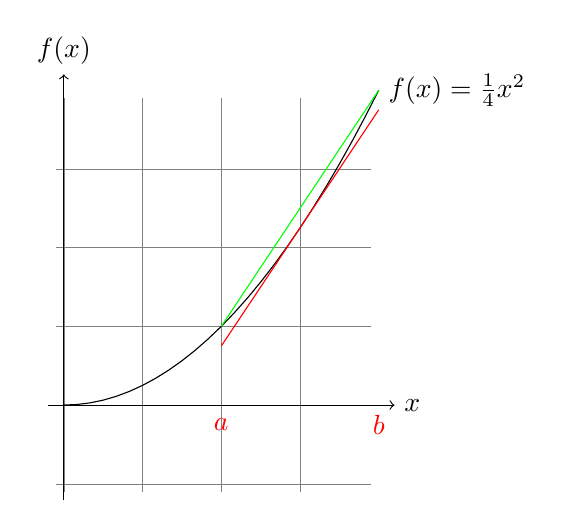
\begin{tikzpicture}[domain=0:4]
    \draw[very thin,color=gray] (-0.1,-1.1) grid (3.9,3.9);
    \draw[->] (-0.2,0) -- (4.2,0) node[right] {$x$};
    \draw[->] (0,-1.2) -- (0,4.2) node[above] {$f(x)$};
    \draw plot (\x,0.25*\x^2) node[right] {$f(x) =\frac{1}{4}x^2$};
    \draw[color=red, domain=2:4] plot (\x,1.5*\x-2.25);
    \draw[color=green, domain=2:4] plot (\x,1.5*\x-2);
    \draw[color=red] (2,-0.25) node {$a$};
    \draw[color=red] (4,-0.25) node {$b$};
\end{tikzpicture}

If a function $f$ is differentiable for $x \in (a,b)$ then there will be a point $x_0$ such that $f(x_0)=\frac{f(b)-f(a)}{b-a}$, meaning that the instantaneous slope at some point will be the average slope of the bounds.

\section{Extreme Value Theorem}

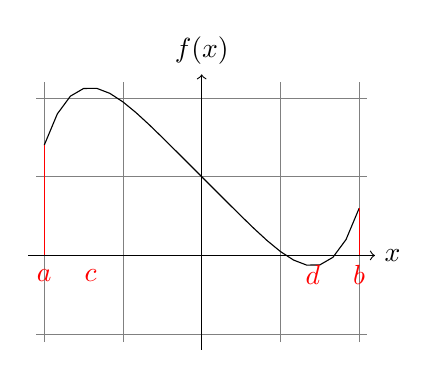
\begin{tikzpicture}[domain=-2:2]
    \draw[very thin,color=gray] (-2.1,-1.1) grid (2.1,2.2);
    \draw[->] (-2.2,0) -- (2.2,0) node[right] {$x$};
    \draw[->] (0,-1.2) -- (0,2.3) node[above] {$f(x)$};
    \draw plot (\x,0.05*\x^5-\x+1) ;
    \draw[color=red] (-2,0) -- (-2,1.4);
    \draw[color=red] (-2,-0.25) node {$a$};
    \draw[color=red] (2,0) -- (2,0.6);
    \draw[color=red] (2,-0.25) node {$b$};
    \draw[color=red] (-1.41,-0.25) node {$c$};
    \draw[color=red] (1.41,-0.25) node {$d$};
\end{tikzpicture}

If a function $f$ is continuous for $x \in [a, b]$ then there exists a maximum and minimum $c$ and $d$, respectively. $f(c) \leq f(x) \leq f(d)$ \textbf{exists.}

\section{Intermediate Value Theorem}

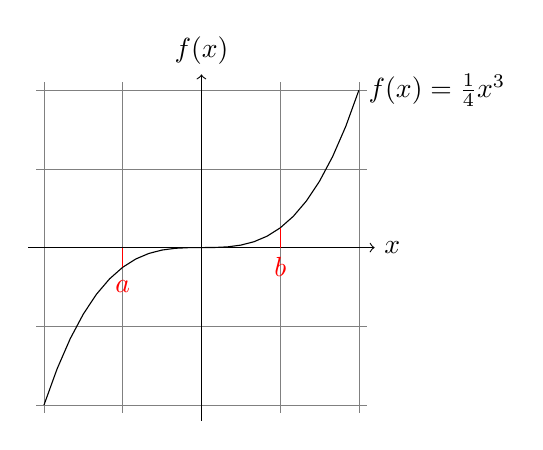
\begin{tikzpicture}[domain=-2:2]
    \draw[very thin,color=gray] (-2.1,-2.1) grid (2.1,2.1);
    \draw[->] (-2.2,0) -- (2.2,0) node[right] {$x$};
    \draw[->] (0,-2.2) -- (0,2.2) node[above] {$f(x)$};
    \draw plot (\x,0.25*\x^3) node[right] {$f(x) =\frac{1}{4}x^3$};
    \draw[color=red] (-1,0) -- (-1,-0.25);
    \draw[color=red] (-1,-0.5) node {$a$};
    \draw[color=red] (1,0) -- (1,0.25);
    \draw[color=red] (1,-0.25) node {$b$};
\end{tikzpicture}

If $f$ is continuous, then there exists a $x$ for $f(a) \leq f(x) \leq f(b)$.

\end{document}
